\documentclass{article}
\usepackage{authblk} % Agrega afiliaciones
\usepackage[english]{babel}
\usepackage{hyperref}
\usepackage{float}
\usepackage[utf8]{inputenc} % Forza encoding en utf8
\usepackage{natbib} % Importa bibliografía
\usepackage{caption,ragged2e,tabularx}
\usepackage{graphicx}
\usepackage{pythontex}

\renewcommand{\figurename}{Figura}
%\decimalpoint

\title{Estimation of remaining individuals by area in Socorro Island \\
    \Large{Feral cat eradication project in Socorro Island, Revillagigedo National Park, Mexico}}
\author{Fernando Alvarez}
\author{Maritza Bello}
\author{Braulio Rojas}
\affil{Data Science Direction}

\begin{document}

\begin{pycode}
import json

ruta_json_simulacion = 'non-tabular/json_meses_faltantes.json'
with open(ruta_json_simulacion, encoding='utf8') as archivo_simulacion:
    meses = json.load(archivo_simulacion)
ruta_json_p_valor = 'non-tabular/json_p-valor.json'
with open(ruta_json_p_valor, encoding='utf8') as archivo_p_valor:
    p_valor = json.load(archivo_p_valor)
\end{pycode}

\maketitle
\begin{abstract}
   According to the data up to September 2019, we determined that: 1) the most probable amount of 
   the remnant cats is \py{'%.0f'% p_valor['gatos_remanentes']} 
   individuals; and 2) considering an effort similar to the latest trends and consider an increase 
   rate equal to zero, we will complete eradication in September 2020. When we consider the 
   intrinsic monthly rate of increase of $r=0.08$ and the carrying capacity of $K=$\py{'%.0f'% meses['capacidad_carga'][0]} 
   cats,  eradication will take \py{'%.0f'% meses['meses_faltantes_k_baja']} months.
\end{abstract}


\section*{Current status}

Following the methodology proposed by Ramsey (2011) and using data from the feral cat eradication 
project on Socorro Island until September 2019, we estimate that the initial population size was 
\py{p_valor['gatos_capturados']+p_valor['gatos_remanentes']} cats. To date, 
\py{'%.0f'% p_valor['gatos_capturados']} 
cats have been removed and the most probable number of remaining individuals is  
\py{'%.0f'% p_valor['gatos_remanentes']} 
cats. 

\begin{table}[H]
\centering
\caption{\small{Current eradication status}}
\label{table:esfuerzoCapturas}
\begin{tabular}{ |c|c|c| }
    \hline
    Current & Percentage & Cats \\
    \hline
    Initial population size & 100\% & \py{'%.0f'%(p_valor['gatos_capturados']+p_valor['gatos_remanentes'])} \\
    Cumulative number of cats removed & \py{'%.2f'% ((p_valor['gatos_capturados']*100)/(p_valor['gatos_capturados']+p_valor['gatos_remanentes']))} \% & \py{'%.0f'% p_valor['gatos_capturados']} \\
    Remaining cats & \py{'%.2f'%((p_valor['gatos_remanentes']*100)/(p_valor['gatos_capturados']+p_valor['gatos_remanentes']))}\%     &  \py{'%.0f'% p_valor['gatos_remanentes']} \\
    \hline
\end{tabular}
\end{table}

\section*{Results}

\begin{figure}[H]
    \centering
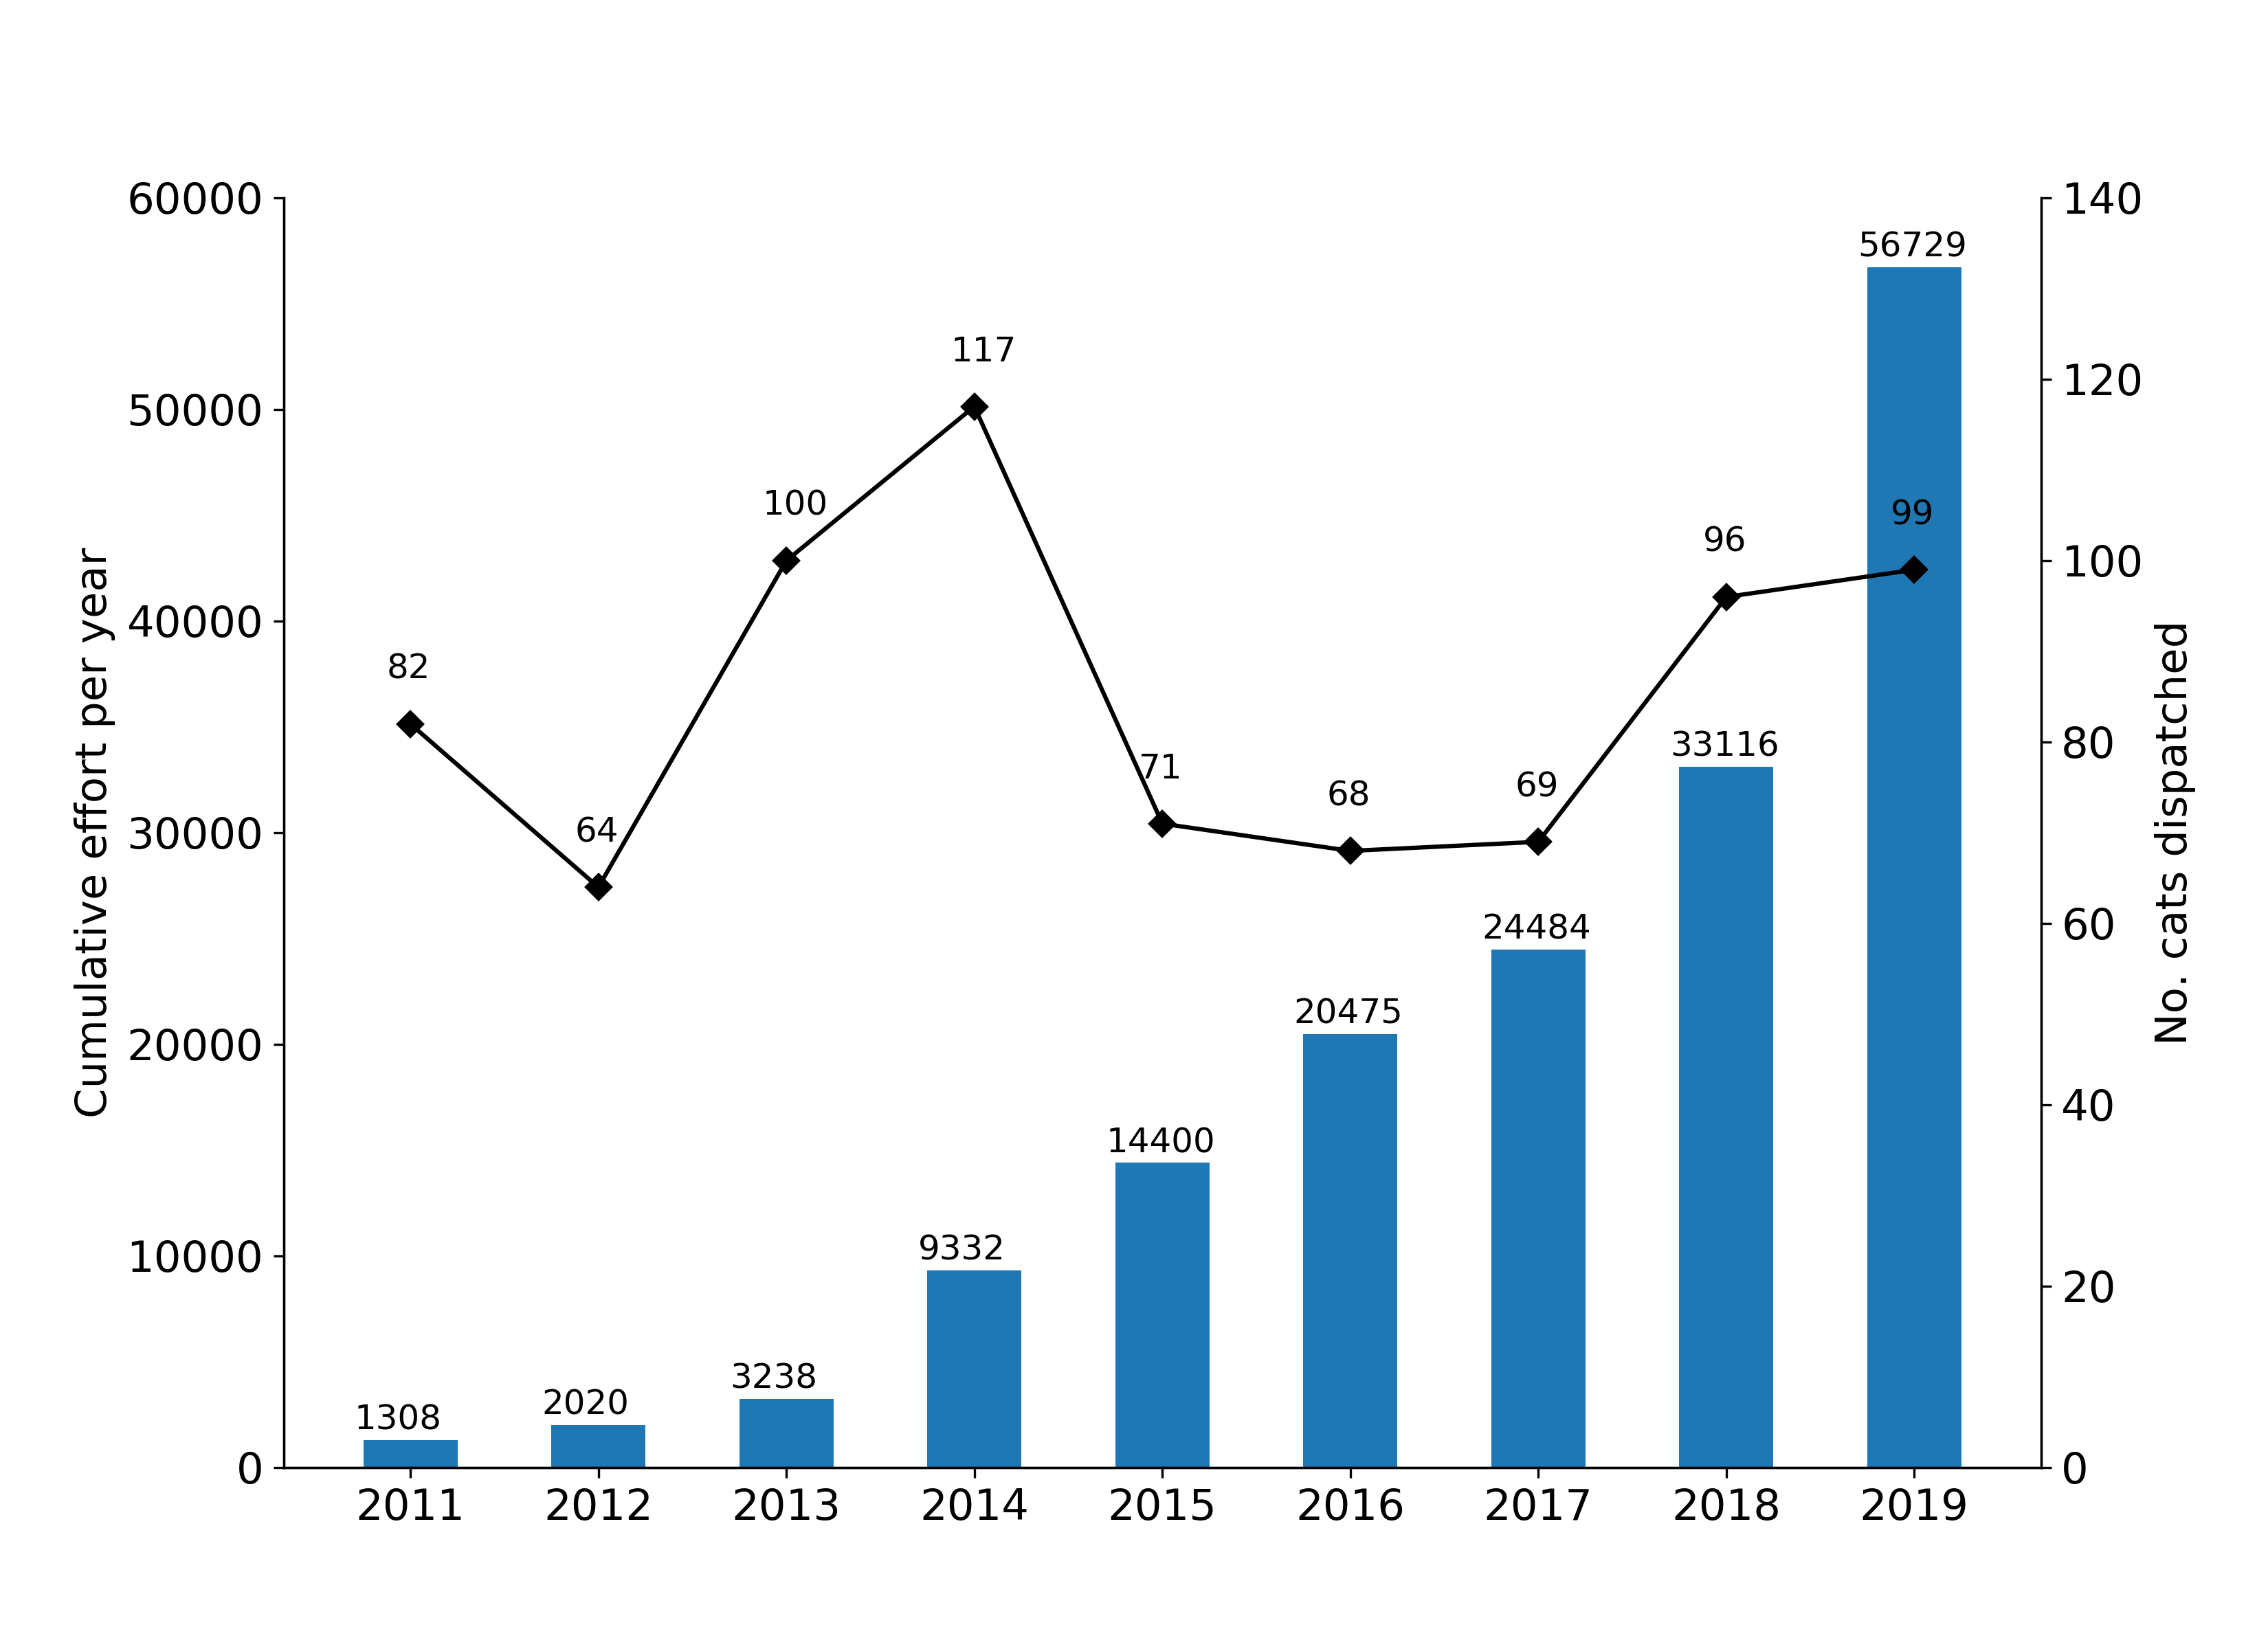
\includegraphics[scale=0.5]{figures/TotalCapturasPorAnioGatosSocorro.png}
\caption{Plot bar with the total effort (night-traps) per year.}
\label{fig:histogramaEsfuerzoTotalPorAnio}
\end{figure}


\begin{table}[H]
\centering
\caption{\small{We show the probability of successful eradication ($\textnormal{P}_\textnormal{s}$), amount of remaining individuals and $p$-value associated with the amount of remaning cats.}}
\label{table:individuosRemanentes}
\begin{tabular}{ |c|c|c|c| }
    \hline
    Probability of & Remaining cats & $p$-value \\
    successful eradication ($\textnormal{P}_\textnormal{s}$) & & \\
    \hline
    \py{'%.0f'%p_valor['probabilidades'][0]}\%      &  \py{'%.0f'% p_valor['gatos_remanentes']}  & \py{'%.2f'% (p_valor['probabilidades'][2]/100)} \\
    \hline
\end{tabular}
\end{table}


The table \ref{table:individuosRemanentes} shows: $\textnormal{P}_\textnormal{s}$, 
the amount of remaining individuals, and the $p$-value (level of trust) associated with the amount of remaining individuals.

\begin{table}[H]
\centering
\caption{\small{Carrying capacity assumed and the months that the eradication will take.}}
\label{table:carryingCapacity}
\begin{tabular}{ |c|c| }
    \hline
    Carrying capacity & Months \\
    \hline
    \py{'%.0f'% meses['capacidad_carga'][0]}      &  \py{'%.0f'% meses['meses_faltantes_k_baja']}  \\
    \py{'%.0f'% meses['capacidad_carga'][1]}      &  \py{'%.0f'% meses['meses_faltantes_k_media']}  \\
    \py{'%.0f'% meses['capacidad_carga'][2]}      &  \py{'%.0f'% meses['meses_faltantes_k_alta']}  \\
    \hline
\end{tabular}
\end{table}

\section*{Conclusion}

\begin{itemize}
\item To complete eradication by January 2020, an effort of 30000 night-traps each month must be applied. That means 34 trappers (with 30 traps each) need to be deployed
\item  TARGET: To complete eradication by July 2020, an effort of 10000 night-traps each month must be applied. That means 12 trappers (with 30 traps each) need to be deployed.
\item If current effort from the last expeditions is maintained (7825 night-traps), we will complete eradication in September 2020.
\end{itemize}	

\section*{Referencias}

Ramsey, D. S., Parkes, J. P., Will, D., Hanson, C. C., and Campbell, K. J.
(2011). Quantifying the success of feral cat eradication, san nicolas island,
california. New Zealand Journal of Ecology, 35(2):163–173.
\end{document}
